\documentclass[doc,12pt]{apa6}
\usepackage[utf8]{inputenc}
\usepackage{enumitem}
\usepackage{environ}
\usepackage{tikz-qtree}

\usepackage{gb4e}

\makeatletter
\newsavebox{\measure@tikzpicture}
\NewEnviron{scaletikzpicturetowidth}[1]{%
  \def\tikz@width{#1}%
  \def\tikzscale{1}\begin{lrbox}{\measure@tikzpicture}%
  \BODY
  \end{lrbox}%
  \pgfmathparse{#1/\wd\measure@tikzpicture}%
  \edef\tikzscale{\pgfmathresult}%
  \BODY
}
\makeatother

\title{Homework 4}
\shorttitle{Homework 4}
\author{Edward Hernandez}
\date{October 2016}
\affiliation{Syntax}

\begin{document}
\maketitle

\section{Part 1}

\subsection{1}

\begin{enumerate}[label=(\alph*)]
	\item The antecedent `the president' does not bind the pronoun `him.' It
		cannot, because, on Condition B, the antecedent of a pronoun cannot
		c-command it if it's within the same clause.
\end{enumerate}

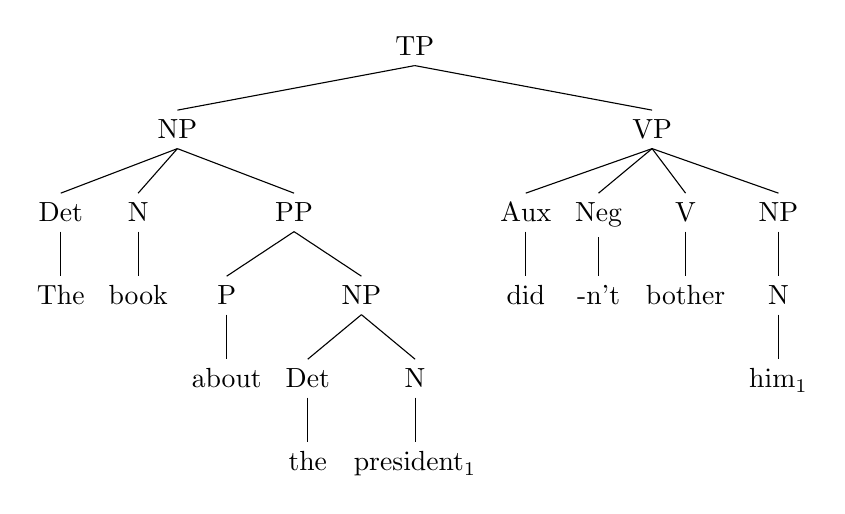
\begin{tikzpicture}
    \Tree [.TP [.NP [.Det The ] [.N book ] [.PP [.P about ] [.NP [.Det the ] [.N president\textsubscript{1} ] ] ] ] [.VP [.Aux did ] [.Neg -n't ] [.V bother ] [.NP [.N him\textsubscript{1} ] ] ] ]
\end{tikzpicture}

\begin{enumerate}[label=(\alph*),resume]
    \item `The book about the president' does not bind `him' because they do not corefer.
\end{enumerate}

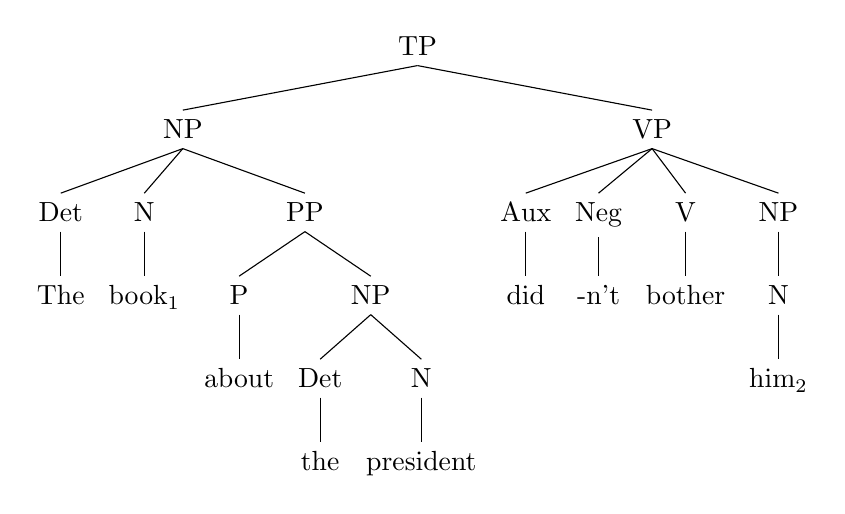
\begin{tikzpicture}
    \Tree [.TP [.NP [.Det The ] [.N book\textsubscript{1} ] [.PP [.P about ] [.NP [.Det the ] [.N president ] ] ] ] [.VP [.Aux did ] [.Neg -n't ] [.V bother ] [.NP [.N him\textsubscript{2} ] ] ] ]
\end{tikzpicture}

\begin{enumerate}[label=(\alph*),resume]
    \item `The book about the president' binds `itself.'
\end{enumerate}

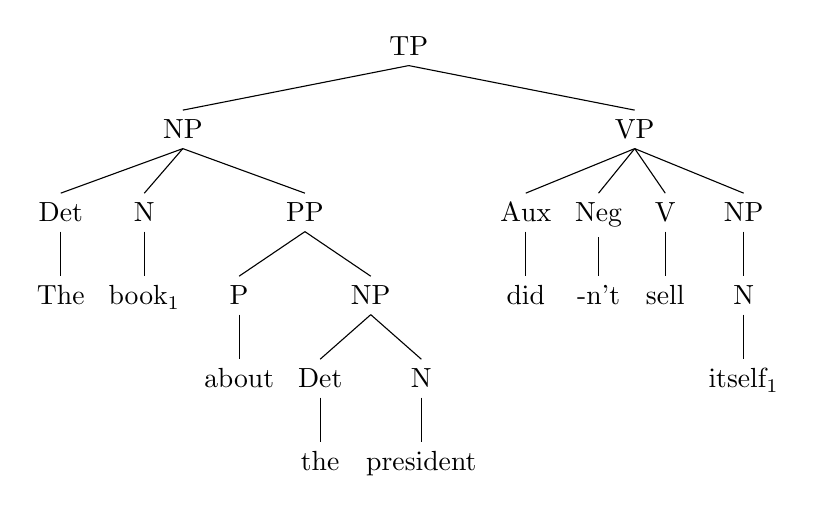
\begin{tikzpicture}
    \Tree [.TP [.NP [.Det The ] [.N book\textsubscript{1} ] [.PP [.P about ] [.NP [.Det the ] [.N president ] ] ] ] [.VP [.Aux did ] [.Neg -n't ] [.V sell ] [.NP [.N itself\textsubscript{1} ] ] ] ]
\end{tikzpicture}

\begin{enumerate}[label=(\alph*),resume]
    \item `The president' binds `his.'
\end{enumerate}

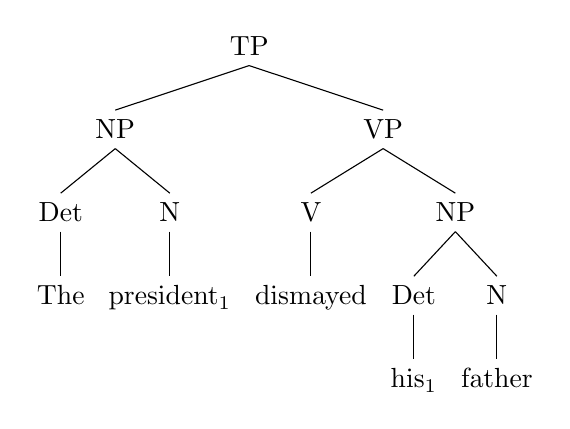
\begin{tikzpicture}
    \Tree [.TP [.NP [.Det The ] [.N president\textsubscript{1} ] ] [.VP [.V dismayed ] [.NP [.Det his\textsubscript{1} ] [.N father ] ] ] ]
\end{tikzpicture}

\subsection{2}

\begin{exe}
    \ex[*]{He\textsubscript{1} likes John\textsubscript{1}.\\
		Condition B is violated because `He' must be locally free.}
    \ex[*]{John's\textsubscript{1} father likes himself\textsubscript{1}.\\
		Condition A is violated.}
    \ex[*]{[John's father]\textsubscript{1} likes him\textsubscript{1}.\\
		Condition B is violated because `him' must be locally free..}
    \ex[*]{John thinks that Bill\textsubscript{1} likes him\textsubscript{1}.\\
		Condition A is violated because `John' is not within the same clause as the anaphor `himself.'}
    \ex[*]{A man that Sally\textsubscript{1} knows adores herself\textsubscript{1}.\\
		Condition B is violated in that `Sally' is not within the same clause as the anaphor `herself'.}
    \ex[*]{[A man that Sally knows]\textsubscript{1} adores him\textsubscript{1}.\\
		Condition B is violated in that a pronoun, `him,' cannot be bound by a local antecedent.}
    \ex[*]{He\textsubscript{1} said that [a man that Sally knows]\textsubscript{1} adores puppies.\\
		Condition C is violated in that `a man that Sally knows,' an R-expression, may not be bound.}
\end{exe}

\section{Part 2}

\subsection{3}

Number agreement in English seems intuitively to be constrained by c-command. A
verb agrees in number with a licensing noun which c-commands it.  As shown in
(10) and (11), this verb does not have to be local to the licensing noun.
\begin{exe}
	\ex{He likes the men.}
	\ex[*]{He like the men.}
	\ex{He likes the men who speak at the meeting.}
	\ex[*]{He likes the men who speaks at the meeting.}
\end{exe}
However, it appears to be the case that verbs are licensed by noun phrases,
rather than individual nouns.
\begin{exe}
	\ex{John and Bill eat.}
	\ex[*]{John and Bill eats.}
\end{exe}
These NPs must still c-command the VP containing which agrees with them.

\subsection{4}

\begin{exe}
    \ex{I showed John\textsubscript{1} himself\textsubscript{1} (in the mirror).}
    \ex[*]{I showed himself\textsubscript{1} John\textsubscript{1} (in the mirror).}
\end{exe}

These sentences show us that c-command is not the only consideration in
determining the acceptability of a binding relationship. There are two possible
interpretations of the above data: that an antecedent may not precede the
anaphor it binds (which we will later see to be incorrect), or that this
particular sort of binding is unacceptable.

Given the data in (18-20), I argue that something about the particular
predicate is taken into account for binding relationships in English. Namely, a
ditransitive verb does not allow its indirect object to bind its direct object.
Making this sort of restriction dependent on predicate information allows for
specifically \emph{psychological predicates} to allow binding contrary to
precedence and other verbs to disallow it.

\section{Part 3}

\subsection{5}

\begin{exe}
	\ex Which picture of himself does John hate?
\end{exe}

That (16) is acceptable tells us that some binding relationships may be formed
in which an element binds an element which precedes it. As discussed above,
this disallows the most intuitive analysis of (14) and (15). Additionally,
`John' seems to bind `himself' despite being non-local (within an embedded
clause) and not c-commanding it.

Above I argue for the specificity of particular predicates. That does not,
however, help to solve the issue of binding here. To allow that, I posit that
this question is special by virtue of being a wh-question, formed from a
structure like that of (17), in which the binding relationship is clear.
\begin{exe}
	\ex John\textsubscript{1} hates pictures of himself\textsubscript{1}.
\end{exe}

\subsection{6}

As I argue above, (18-20) may be acceptable in virtue of something about the
particular psychological predicates they contain. Beoynd the posibility that
this sort of predicate allows unusual binding relationships, I think it is
reasonable to posit that these sentences may have an underlying structure
something like (21) and then undergo some sort of movement process not unlike
wh-movement, through which binding is preserved.
\begin{exe}
	\ex The pictures of himself worry John.
	\ex Those stories about herself frighten Sue.
	\ex Criticisms of themselves annoy the kids.
	\ex John\textsubscript{1} worries about the pictures of himself\textsubscript{1}.
\end{exe}
This explains the unacceptability of (22-24), as they are not acceptable even 
in the unmoved structure, as in (25).
\begin{exe}
	\ex[*]{The pictures of himself worry John's mother.}
	\ex[*]{Those stories about herself frighten Sue's mother.}
	\ex[*]{Criticisms of themselves annoy the teacher of those kids.}
	\ex[*]{John's mother worries about the pictures of himself.}
\end{exe}

\end{document}
